\section{Conclusion}\label{sec:ciConclusion}


A search for new non-resonant dilepton production in the dielectron and dimuon invariant-mass spectra has been presented.
This search made use of the full 139 fb$^{-1}$ of proton--proton collision data collected by ATLAS during Run~2 of the LHC at $\sqrt{s}=13$~TeV.
No significant excess is observed above the expected background.
Upper limits are set on the \xsbr of new signal processes and lower limits on the CI scale \lam.
The limits on \xsbr are easily reinterpreted in terms of new physics models.
This is the first time such results have been made available.
The limits on \lam are the most robust frequentist limits ever set on contact interaction models.

% Improvements
A number of new techniques were developed in order to enable the production of this result.
% Data driven
Most significantly, the results make use of a background estimate derived from the data in a low mass control region.
This approach replaces theoretical and experimental uncertainties with well studied statistical uncertainties on the background estimate.
These uncertainties are measured directly and robustly.
In particular, a new method for measuring spurious signal has been introduced with the ISS procedure.
% Frequentest
Additionally, the limits on both \xsbr and \lam are set using a frequentist approach.
This eliminates arbitrary prior probabilities on signal models.
These techniques, along with the integrated luminosity of the full Run~2 dataset, allow this search to probe unprecedented energy and length scales.
The strongest limits are set on the combined left-left chirality constructive model.
These observed (expected) limits exclude this model for \lam up to 35.8(27.6)~TeV at 95\% CL.

\begin{figure}[h!]
\centering
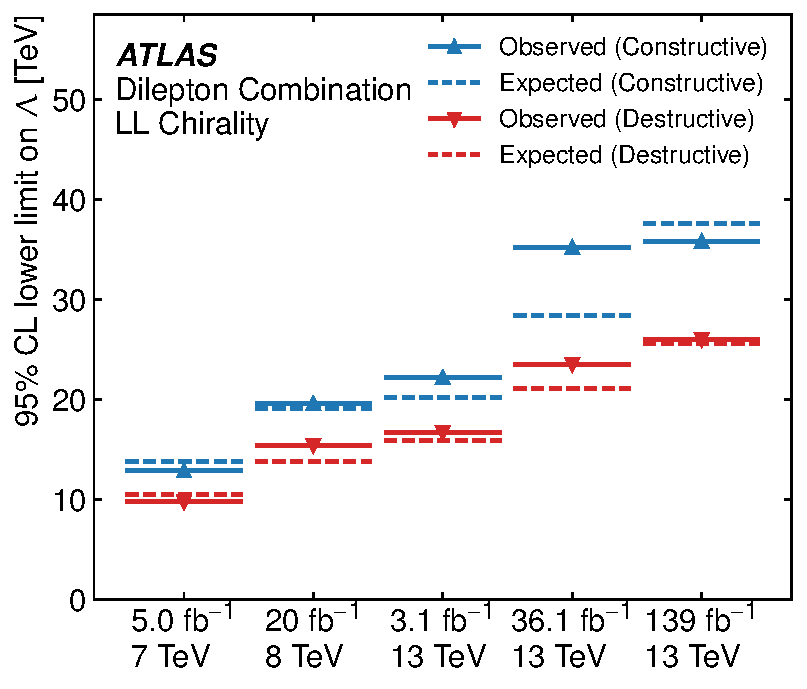
\includegraphics[width=0.70\textwidth]{figures/ci/results/figaux_05.pdf}
\caption{Comparison of the $\ell\ell$ constructive (blue) and destructive (red) LL chirality limits with previous ATLAS results. For results with Bayesian limits, the $\Lambda^{-4}$ prior is used. ($\sqrt{s}=13$~TeV 36.1 fb$^{-1}$ result: \cite{EXOT-2016-05}, $\sqrt{s}=13$~TeV 3.1 fb$^{-1}$ result: \cite{EXOT-2015-07}, $\sqrt{s}=8$~TeV 20 fb$^{-1}$ result: \cite{EXOT-2013-19}, $\sqrt{s}=7$~TeV 5.0 fb$^{-1}$ result: \cite{EXOT-2012-17}.)}
\label{fig:ciHistoricalLimits}
\end{figure}

The results of this analysis are placed in context in Figure \ref{fig:ciHistoricalLimits}.
Here the evolution of ATLAS results is shown using various collision energies and luminosities.
The results are arranged chronologically based on their publication.
The steady progression of the expected limits can be seen over time, and the left-left chirality results of this analysis appear in the final bin.


